\section{Literaturrecherche}

Die Erzeugung von Energie mittels Photovoltaik spielt global und in Deutschland eine immer größere Rolle. \n
Sowohl im privaten Bereich auf Gebäudedächern als auch in größeren zentralen Anlagen wird Energie produziert
und eingespeist.\\
Nach dem Bundesministerium  für Wirtschaft und Energie werden 6.1\% des deutschen\\ Strombedarfs durch Solarenergie gedeckt (Abb. 1).
Die Energiegewinnung erfolgt durch das Potential über ein Halbleitergitter, z.Bsp. einem aus Silizium.
In dieses Silizium besteht aus 2 Schichten. Die eine Schicht ist durchsetzt mit Elektronendonatoren, die andere mit Elektronenakzeptoren. Diese Schichten nennt man n- bzw. p-Schicht.\\ Am Übergang zwischen den beiden Schichten legen sich die überschüssigen Elektronen aus der n-Schicht locker an die Elektronenakzeptoren der p-Schicht an. So entsteht ein elektrisches Feld. Photonen treffen auf diese Schicht und lösen diese gebundenen Elektronen ab. Das elektrische Feld bewegt sie nun zurück zur n-Schicht.\\ Sie gelangen dort zu Kontakten in den äußeren Stromkreis. Dort können sie als elektrische Leistung verwendet werden. \cite{WdP}\\
Wichtig zum Verstehen von Photovoltaik sind 2 Konzepte. Zuerst die sog. IU-Kennlinie. Sie besteht aus 4 Quadranten und beschreibt das Verhalten des Solarpanels als Spannungs/Stromquelle bei Beleuchtung. Aus dem Diagramm kann man sofort sehen, dass es einen Punkt gibt, an dem Strom und Spannung am größten sind
Es gibt jedoch einige Probleme mit Photovoltaik:\\
Die Energieerzeugung hängt direkt mit dem vorhandenen Lichtniveau zusammen.
Eine sinnvolle Speichermöglichkeit wurde noch nicht gefunden. Dies kann zu starken Schwankungen in der Energieproduktion fürs Netz führen - Solarenergie ist also extrem schlecht planbar.
\begin{figure}[b]
    \centering
    \subfloat[\centering label 1]{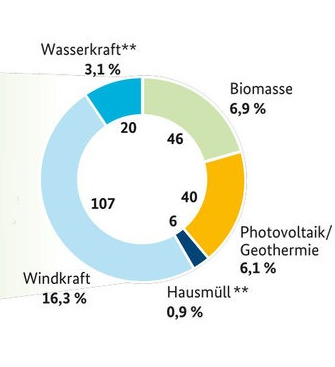
\includegraphics[width = 5cm]{Templates/bruttostromerzeugung-in-deutschland.jpg}}%
    \qquad
    \subfloat[\centering label 2]{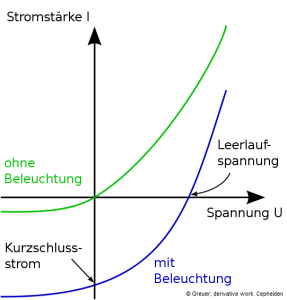
\includegraphics[width = 5cm]{Templates/Kennlinie-287x300.png}}%
    \caption{Zusammensetzung regenerativer Strom und typische IU-Kennlinie \cite{photovoltaik.com}}%
\end{figure}


